\documentclass[a4paper, 10pt,  twocolumn]{ltjsarticle}

% 画像
\usepackage[dvipdfmx]{graphicx}
% 表
\usepackage{booktabs}
\usepackage{enumerate}

% 数式
\usepackage{amsmath}
\usepackage{amssymb}
\usepackage{amsfonts}

\usepackage{multicol}
\usepackage{lipsum} % ダミーテキスト用


% ベクトル
\usepackage{bm}
% コード
\usepackage{listings,jvlisting}
% コードの色
\usepackage{color}
\usepackage{subcaption}
\usepackage{array}

\definecolor{OliveGreen}{rgb}{0.0,0.6,0.0}
\definecolor{Orenge}{rgb}{0.89,0.55,0}
\definecolor{SkyBlue}{rgb}{0.28,0.28,0.95}
% ここからコードの表示に関する設定
\lstset{
  language=C++,
  basicstyle={\ttfamily},
  identifierstyle={\small},
  commentstyle={\small\itshape},
  keywordstyle={\small\bfseries},
  ndkeywordstyle={\small},
  stringstyle={\small\ttfamily},
  frame={tb},
  breaklines=true,
  columns=[l]{fullflexible},
  numbers=left,
  xrightmargin=0zw,
  xleftmargin=3zw,
  numberstyle={\scriptsize},
  stepnumber=1,
  numbersep=1zw,
  lineskip=-0.5ex,
  keepspaces=true,
  keywordstyle={\color{SkyBlue}},
  commentstyle={\color{OliveGreen}},
  stringstyle=\color{Orenge},
  showstringspaces=false
}
\renewcommand{\lstlistingname}{Code}
\newcommand{\E}[1]{\times10^{#1}}



\title{人工知能 中間レポート 課題5}
\author{03420414  小松麟太郎}
\date{\today}


\begin{document}

\maketitle

\section{序論}
本レポートでは人工蜂コロニーアルゴリズム（Artifitial Bee Colony, ABC）を用いて，3次元のHP構造予測問題を解くプログラムを作成した．
\section{アルゴリズム}
\subsection{HP構造の表現}
HP構造をABCを適用できる形で表現するために，hintの論文[1]の方法を用いた．この方法では，HP構造を各アミノ酸の相対的な折り畳み方向 S（前），L（左），R（右），U（上），D（下）の配列で表現する（例 : SLDUSLRLLD）．このように表された任意の配列について，次のようにHP構造を決定することができる．\\
\quad まず1，2番目のアミノ酸を互いの距離が1になるように任意の位置に配置する．次に，1番目のアミノ酸から2番目のアミノ酸への伸長方向の単位ベクトルを $\boldsymbol{x}$ として, それと直交するように単位ベクトル $\boldsymbol{y}$ ，さらに $\boldsymbol{z} = \boldsymbol{x}\times\boldsymbol{y}$ をとり，3つのベクトル，$\boldsymbol{x}$，$\boldsymbol{y}$，$\boldsymbol{z}$ を軸とするローカル座標系を定義する．このとき，S を $\boldsymbol{x}$，L を $\boldsymbol{y}$，R を $-\boldsymbol{y}$，U を $\boldsymbol{z}$，D を $-\boldsymbol{z}$ として，2番目のアミノ酸の位置から折り畳み方向の配列の最初の要素のベクトル方向に1進んだ位置に3番目のアミノ酸を配置する．そして，3番目のアミノ酸の伸長方向に $\boldsymbol{x}$ が重なるようローカル座標系を回転させ，これを3番目のアミノ酸のローカル座標系として4番目のアミノ酸の位置を決定する．この操作を繰り返すことで，与えられた折りたたみ方向の配列から，各アミノ酸の位置が決まり，最終的なHP構造を一意に決めることができる．3次元でなく2次元で最適化する場合は，折り畳み方向を S（前），L（左），R（右）の3つだけ考えるようにすれば，同様にしてS, L, Rの配列から構造を決定することができる．
\subsection{ABCを用いた最適化}
ABCを用いた最適なHP構造の探索手順を説明する．
\subsubsection*{(1) 初期化}
Employed beeと Onlooker bee の個体数を $N$ とする．探索点として $N$ 個の折り畳み方向配列を個体に持つ $A = \{\boldsymbol{a}_1,\cdots, \boldsymbol{a}_N\}$ をランダムに生成する．$\boldsymbol{a}_i$ の水素結合の数を $f_i$ とする．Employed bee が $\boldsymbol{a}_i$ を更新しなかった回数 $s_i$ を $0$ とする．
\subsubsection*{(2) Employed bee の探索}
Employed bee の探索では，0 から $N$ までのすべての探索点を1度ずつ更新する．講義で紹介されたABCアルゴリズムにおける更新法は，以下のとおりである．\\
\textbf{講義で紹介された方法}
\begin{itemize}
    \item 探索点$i$を更新するとき，更新する次元$m$及び$i$と異なる探索点$j$をランダムに選ぶ．
    \item 以下の式で点の更新候補$\boldsymbol{a}'_i$を計算する．（$\boldsymbol{a}_i$は元の個体、次元$m$以外は$\boldsymbol{a}'_i$は$\boldsymbol{a}_i$と同じ）．
    \begin{equation}
        a'_{i, m} = a_{i, m} + \mathrm{rand}(-1, 1)(a_{i, m}-a_{j, m})
    \end{equation}
    \item $\boldsymbol{a}'_i$ での水素結合の数 $f'_i$ が $f_i$ より大きければ探索点 $i$ の個体を$\boldsymbol{a}'_i$に更新し，$s_i$を0にする．更新されなかった場合$s_i$に1を足す．
\end{itemize}
スライドの方法では，式（1）要素同士の演算をしているが，で2.1で定義した折り畳み方向配列は要素の種類がS，L，R，U，D の5つで有限なので，そのような演算を定義するのは難しい．そこで次のように遺伝的アルゴリズムの交叉のような方法で配列を更新するようにした．また，各個体を交叉させる際に，2つの構造同士を組み合わせる向きを全探索し，最も水素結合が多いものを採用するというようにした．これは，遺伝的アルゴリズムを用いてHP構造予測問題を解いている[2]の考え方に基づいている．[2]では単一交叉を用いていたが，2点交叉にした方が良い結果が得られたので，本アルゴリズムでは2点交叉を採用した．\\
\textbf{使用した方法}
\begin{itemize}
    \item 探索点$i$を更新するとき, $i$と異なる探索点$j$をランダムに選ぶ．
    \item ランダムに交叉点の次元 $m$, $n$, $(m < n)$ を選び，$\boldsymbol{a}_i$ の $ m,\cdots,n $ の次元を $\boldsymbol{a}_j$ のものに置き換えた個体を $\boldsymbol{a}'_i$ とする．さらに$\boldsymbol{a}'_i$ の次元 $m$, $n$ の要素 $a'_{i, m}$, $a'_{i, n}$ を S, L, R, U, D に変えた場合の水素結合の数をすべての組み合わせに対して計算し，その中で水素結合が最も多い個体を $\boldsymbol{a}''_i$ とする．
    \item $\boldsymbol{a}''_i$での水素結合の数 $f''_i$  が$f_i$より大きければ，探索点 $i$ の個体を$\boldsymbol{a}''_i$に更新し，$s_i$を0にする．更新されなかった場合$s_i$に1を足す．
\end{itemize}

\subsubsection*{(3) Onlooker bee の探索}
Onlooker bee の探索では，水素結合の数 $f_i$ から探索点 $i$ が選ばれる相対確率 $p_i$ を，
\begin{equation}
    p_i = \frac{f_i+1}{\sum_{k = 1}^{N} (f_k+1)}
\end{equation}
この相対確率を利用して，探索点 $i$ を選び，Employed bee の探索と同じ手順で探索点を更新する．
\subsubsection*{(4) Scout bee の探索}
更新されなかった回数 $s_i$ がある上限 $s_{\mathrm{max}}$を超えた場合，探索点 $i$ の Employed bee は Scout bee となる．この場合，探索点 $i$ の個体をランダムに生成した個体に変え，$s_i = 0$ とする．

\subsubsection*{(5) 終了処理}
（2）から（4）のプロセスを与えられた世代数分繰り返した後，水素結合の数の最も多い個体を結果として出力する．
\section{実装}
今回のアルゴリズムの実装には，C$++$を用いた．また，プログラムを実行して得られた2次元ないしは3次元の構造をわかりやすい形で表示するために OpenGL を用いた．OpenGLのプログラムは後期実験のOpenCV/GL演習で用いたものをほぼ流用した．世代数，個体数，$s_\mathrm{max}$ ，HP配列を入力すると最適構造を計算した後，得られた構造が図1のように表示される．青の球体が親水性アミノ酸(H)，赤の球体が親水性アミノ酸(P)，赤色の線で表される結合がアミノ酸同士のペプチド結合，青の点線で表される結合が水素結合である．
\begin{figure}[t]
    \centering
    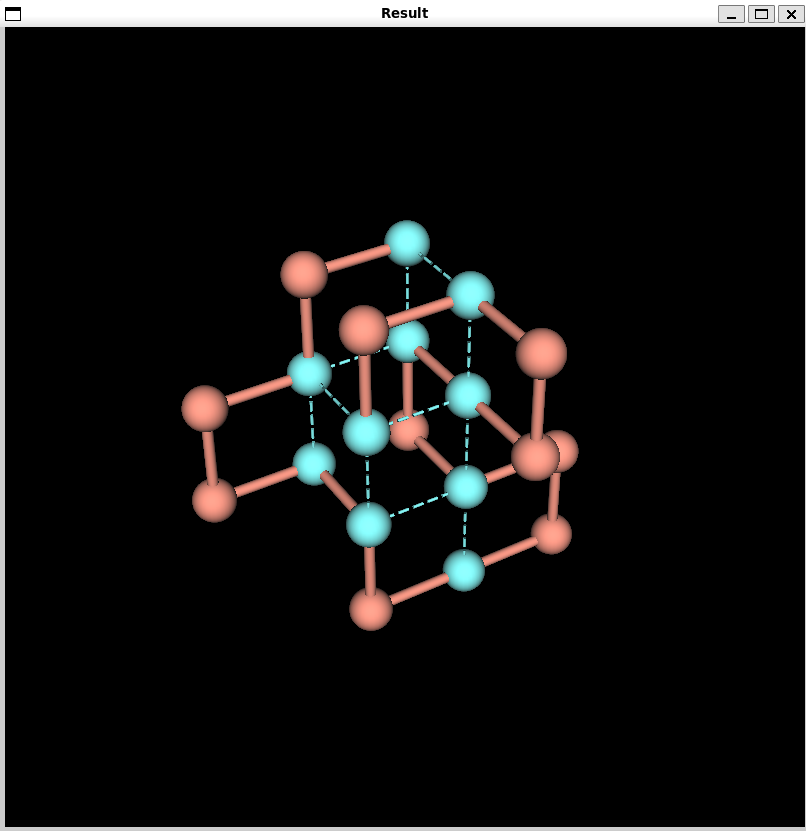
\includegraphics[width=0.8\linewidth]{image1.png}
    \caption{ 長さ20のHP構造の表示}
\end{figure}
\section{結果}
以上で説明したアルゴリズムを用いて，課題で与えられた表1に示す5つの配列について最適構造を計算した．プログラムの実行環境は以下のとおりである.

\begin{table*}[t]
    \centering
    \begin{tabular}{@{}ccl@{}}
        \hline
        番号 & 長さ & 配列 \\\hline
        (1) & 20 & (HP)2PH2PHP2HPH2P2HPH \\
        (2) & 48 & P2HP2H2P2H2P5H10P6H2P2H2P2HP2H5\\
        (3) & 48 & HPH2P2H4PH3P2H2P2HPH2PHPH2P2H2P3HP8H2\\
        (4) & 48 & PHPH2P2HPH3P2H2PH2P3H5P2HPH2(PH)2P4HP2(HP)2\\
        (5) & 48 & PH2P6H2P3H3PHP2HPH2(P2H)2P2H2P2H7P2H2\\
        \hline
    \end{tabular}
    \caption{用いた配列}
\end{table*}
\begin{table*}[t]
    \centering
    \begin{tabular}{@{}cc|cccc|cccc@{}}
        \hline
        && 2次元 &  && & 3次元 & && \\\hline
        配列 & 長さ& 世代数 & 個体数 & 水素結合の数 & 実行時間 & 世代数 & 個体数 & 水素結合の数 & 実行時間  \\\hline
        (1) & 20 & 50 & 100 & 9(9) & 0.2 s & 200 & 300& 11 & 2.7 s \\ 
        (2) & 48 & 300 & 1000 & 23(23) & 15.4 s & 500 & 2000 & 31 & 2.3 min \\ 
        (3) & 48 & 500 & 2000 & 19 & 56.3 s & 500 & 2000 & 30(32) & 2.1 min \\ 
        (4) & 48 & 500 & 2000 & 19 & 54.6 s & 1000 & 4000 & 32(34) & 10.1 min \\ 
        (5) & 48 & 500 & 2000 & 21 & 56.7 s & 1000 & 4000 & 32(33) & 10.3 min \\ 
        \hline
    \end{tabular}
    \caption{実行結果}
\end{table*}
\begin{figure*}[t]
    \centering
    \begin{minipage}{0.45\linewidth}
        \centering
        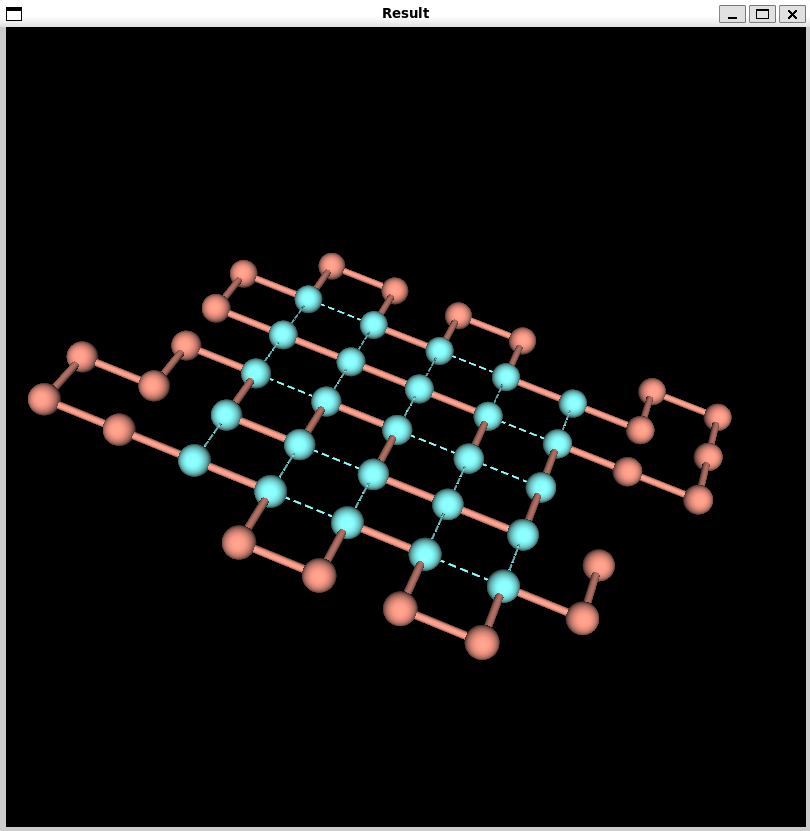
\includegraphics[width=0.8\linewidth]{image2.png}
        \subcaption{2次元 水素結合 : 23個}
    \end{minipage}
    \hfill
    \begin{minipage}{0.45\linewidth}
        \centering
        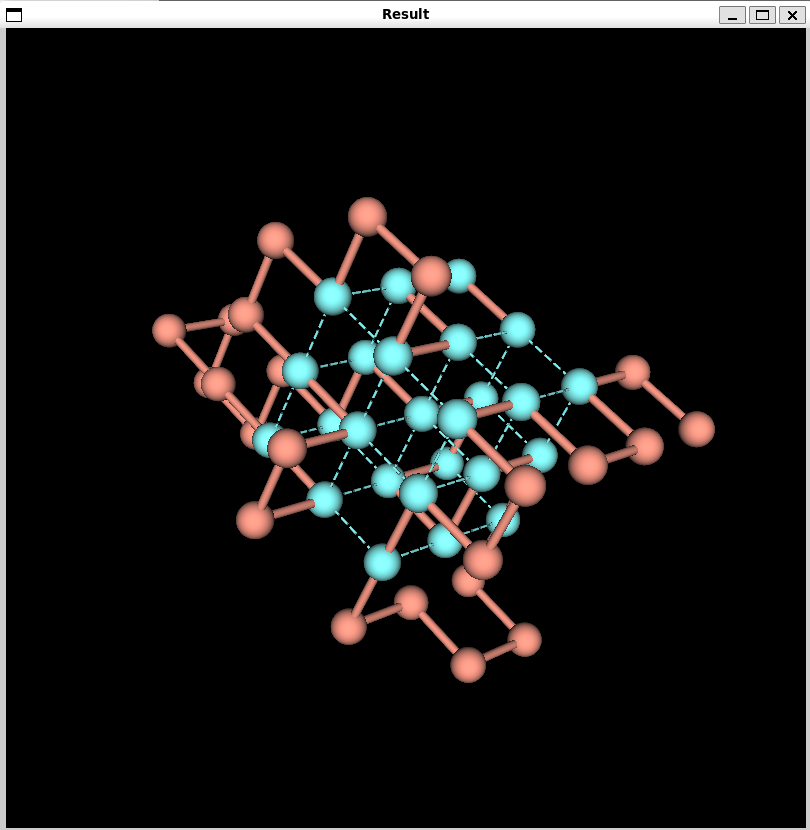
\includegraphics[width=0.8\linewidth]{image3.png}
        \subcaption{3次元 水素結合 : 31個}
    \end{minipage}
    \caption{配列（2）の最適化の結果}
\end{figure*}
\begin{itemize}
    \item コンピュータ ：NEC PC-XC75ODAG
    \item OS ： WSL2 Ubuntu 22.04.06 LTS
    \item CPU ：11th Gen Intel Corei7-1195G7 
    \item メモリ ： 16GB 
\end{itemize}
表2は表1の入力配列に対して，2次元と3次元での最適化したときの，得られた水素結合の数，実行時間を表したものである．水素結合の数の()内の値は最適な構造の水素結合の真の数を示している[1]． $s_{\mathrm{max}}$ の値は 50 に固定した．どの配列についても2次元から 3次元にすることによって水素結合の数が増大していることが分かる．表から配列（1），（2）については，2次元では真の最適構造を見つけられたが，配列（2），（3），（4）については，3次元で真の最適構造を見つけ出すことができなかった．一方で[1]で提案，比較されている ACO（Ant Colony Optimization）やPERM (Prune and Enriched Rosenbluth Method) による最適化においては，これらの配列の3次元構造について真の最適構造を見つけ出すことができている．このことから，これらの手法は本レポートのABCによる手法より優れているといえる．ただ，本レポートで提案したABCによる手法においても，世代数や個体数，$s_i$ のパラメータについてはあまり考察ができていないので，まだ改善の余地があると考えられる．

\begin{thebibliography}{99}
    \item
    Shmygelska, A., Hoos, H.H. An ant colony optimisation algorithm for the 2D and 3D hydrophobic polar protein folding problem. BMC Bioinformatics 6, 30 (2005).
    \item 
    Unger R, Moult J. Genetic algorithms for protein folding
    simulations. J of Mol Biol (1993).
\end{thebibliography}
\end{document}
